\chapter{Research}
Throughout this chapter, I will be investigating how networking is implemented in popular modern AAA games. I will also implement a simple online, multiplayer demo game using different ways of implementing networking in the Unity game engine. The experience of using the options that exist in Unity for network game developement, will be similar to what I will aim to implement at a much lower level with my networking template.

\section{Networking implementations in games}
TODO:

\subsection{Variable ping system in Battlefield 1}
An interesting approach to the issue of variable ping in a game has been implemented by DICE in the game Battelfield 1. Given 2 players; player A with a low ping to the server and player B with a ping of <150ms to the server.

When player B fires at a moving player A, player B's client will perform the check concluding that player A has been hit and this information is sent to the server. The server will then perform it's own checks and if the server agrees that this hit is possible, then it sends the hit confirmation to player B and damage information to player A. This approach is called Clientside-Server Authoritative as while the hit registration is calculated on clientside, the server must still confirm that this is valid.

Concidering another scenario, suppose that player A still has a low ping to the server but player B, now has the ping of >150ms. An icon will appear on player B's UI showing an ``aim-lead'' indicator. Now when the shot is fired in the same scenario, the hit will not register anymore as the hit registration has switched from Clientside-Server Authoritative to Fully-Server Authoritative, meaning that the check is performed only once the shot information is received by the server.

Whilest this implementation makes the game feel less responsive for players with high ping, it provides a lot more fairness for everyone else and allow for players with different pings play in a more fair way.


\subsection{Networking in Apex Legends}
Apex Legends is a ``Battle Royale'' game by Respawn Entertainment. Due to the genre of this game, the implementation of networking has been implemented in an interesting way. The premise of the game consists of a starting amount of 60 players, all competing to be the last one alive at the end. An interesting aspect of this, is that while at the start of a match, the server might have to work quite hard to effectively synchronise the simulation for 60 different clients, as more and more players die off and less are left, less information needs to be sent to each of the clients, freeing up some server performance.

Since transferring all the information about 60 different players would most likely exceed the average MTU of a UDP packet, with each update, the server sends 1 smaller packet per each player to each player. This means that when 60 players are in the game, 60 packets are sent to 60 different clients from the same server. This is shown in the Netcode analysis in \mycite{bns2019apex}.

An interesting outcome of this, is quite noticible network lag that slowly goes away, as less and less players remain in the game. It is also likely due to this, that Respawn felt the need to implement a ``Client Authoritative'' aiming model. Meaning that the server will favor what the client sees over it's own view of the simulation (i.e. If the client claims that a shot has hit an enemy, the server is likely to agree). The choise for this implementation could have been made to fix two potential issues; reducing the load on the server by reducing the need to perform extencive checks for each shot (this could be significant if a lot of players are playing), making the game feel more responsive on slower client hardware that may need more time to process up to 60 packets that arrive from the server at each update tick.

\subsection{Destiny 2's uniquely complicated netcode}
In 2015, a Bungie developer gave an interseting talk at GDC (Game Developer's Conference): \mycite{truman2015destiny2}. The game Destiny 2, has decided to use the peer to peer model to create an ``always online'' world that players could join and leave freely. This resulted in a netcode that was refered to by \author{truman2015destiny2} as having a  ``uniquely complicated network topology''. In a previous Bungie game with multiplayer networking, Halo Reach,  a mixture of a peer to peer model and client hosted model has been used in multiplayer matches. Each player would send information such as weapon fire or movement to all other players but there would also be a physics server running on one of the clients in the simulation. The matches were designed to be relatively short and players where incentivised to remain in the game until the end of each match. This meant that if the player running the physics server were to leave, the gameplay flow would have to be interrupted for all other players as the host migration system allocated a new player to run this server. Fortunately, due to the nature of the game, this happened rarely as players were incentivised to remain till the end of the match. In Destiny 2 however, there are many zones (refered to in the talk as ``bubbles'') that a players would often join and leave as they move around the environment. This made host migrations much more common and would happen roughly ``every 160 seconds''. This has prompted Bungie to abandon the client hosted physics server aspect of Destiny 2's netcode and move towards renting cloud server space to host the physics engine. In ``private bubbles'', however, it became inefficient to communicate with a central server for game physics calls so the old system was used there. In summary, Destiny 2 uses peer to peer in order to send packets directly to other players to make the gameplay feel more responsive than sending messags to the server and then a client but has fixed some issues that the game could have if it was fully peer to peer by implementing elements that use client hosted and central server models too.

\begin{figure}[!h]
  \centering
  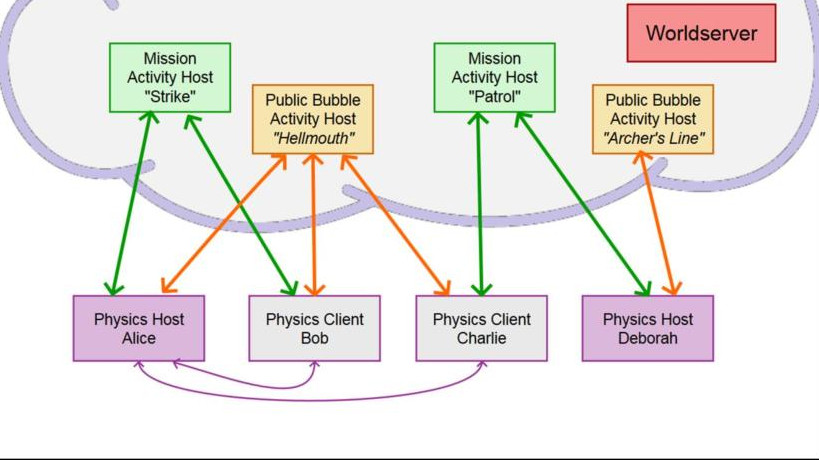
\includegraphics[width=0.5\textwidth]{Destiny2_networking}
  \caption{Example of how netcode is designed in Destiny 2. Image from the GDC talk: \mycite{truman2015destiny2}}
  \label{fig:destiny2netcode}
\end{figure}

\subsubsection{Issues with the peer to peer system}


\newpage
\section{Other networking developement tools}
TODO:

\subsection{Unity's UNET}
Allows for easy implementation of Client Hosted model in Unity. Hard to get working like I wanted.


\subsection{Photon Network in Unity}
Similar to UNET, allows for easy and free server sental for central server model


\subsection{Google's Stadia}
Allows for easy networking since it's already on server
